%This section provides a high-level statement of your product concept - what it is intended to do and how it is intended to be used. Include in this header paragraph, a brief synopsis of what is described here. For example, this header paragraph might say something like: "This section describes the purpose, use and intended user audience for the X product. X is a system that performs Y. Users of X will be able to Z..."
This section describes the purpose, use and intended user audience for the Cerberus. Our product, Cerberus, is a wireless wrist module system that notifies deaf or hard of hearing individuals of events happening around them. The wearer will be notified by the wrist module from a vibration. The vibration signals them to check their phone to see the event description of what triggered the vibration. 

\subsection{Purpose and Use}
%This is where you describe in a brief, yet clear and concise, manner what your product should do and how you expect it should be used.
The Cerberus wrist module is to be worn by the customer. The wrist module will signal the wearer to check their phone when an event happens via a vibration. The Cerberus phone app will receive notifications from the server. The server will communicate with the Ring system and push event notifications from the Ring system to the phone app. Events from the Ring system will include the doorbell being rung, the motion detector being tripped, or the alarm system going off. For the Cerberus system to be used effectively, the customer must have access to a Ring system. 

\subsection{Intended Audience}
%This is where you describe the intended audience(s) of your product. If this product were to be made available publicly or commercially, who would purchase or use it? Is the product designed for a particular customer, or an overall class of customers? Is it intended for general use, or is it a specific component of a more complex system?
Our product is designed for deaf and hard of hearing individuals. This includes members of the deaf community and elderly or regular individuals who suffer from some sort of hard of hearing. The Cerberus package is intended to be used alongside the Ring system, so the audience must have access to Ring products.

\begin{figure}[h!]
	\centering
   	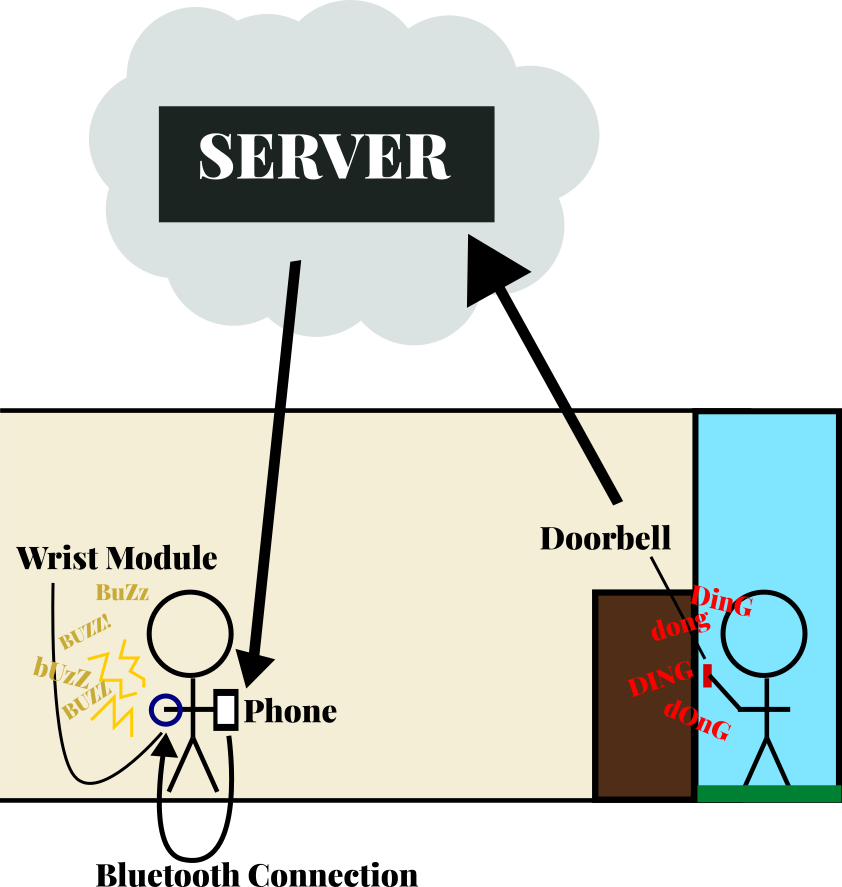
\includegraphics[width=0.60\textwidth]{images/high-level-system-overview.png}
    \caption{Conceptual drawing}
\end{figure}
